% !TEX root = thesis-ex.tex

The hadronic shower (jet) has both electromagnetic and non-electromagnetic components that interact with the calorimeter material differently.
Thus the energy response of the calorimeter for these components is different (this is called a non-compensating calorimeter \cite{calorimetry_book}), and hence, calibrations are required to correct the reconstructed jet kinematics.
These take into account features of the detector, the reconstruction algorithm, and jet fragmentation and include the following \cite{Aad:2014bia}:
\subparagraph{Origin Correction: } This correction ensures that jets point back to the primary vertex and not the nominal center of the detector.
\subparagraph{MC based Calibration: } This is a MC based correction that depends on the comparison between the energy and pseudorapidity of the reconstructed jet and the corresponding matched truth jet.
\subparagraph{\textit{In situ}+Cross Calibration: } This calibration is based on the differences between data and MC as described by a well-measured object like a photon or Z boson.
This poses a challenge for heavy ion collisions because unlike in \pp\ collisions, there simply aren't enough statistics for these objects.
Here the cross-calibration procedure accounts for differences in the jet reconstruction procedure in heavy ion collisions and \pp\ collisions, and enables the usage of the \insitu\ corrections from \pp\ collisions.

The validity of the jet reconstruction and calibration procedure can be tested by evaluating the jet energy scale and jet energy resolution.
These are the mean and width respectively of the jet response distribution that is given by $\ptreco / \pttruth$ in MC and are shown in Figure~\ref{fig:jes_jer}.
\ptreco\ is the reconstructed jets transverse momentum, while \pttruth\ is the transverse momentum of the corresponding ``truth'' jet.


\begin{figure}[htbp!]
	\centering
	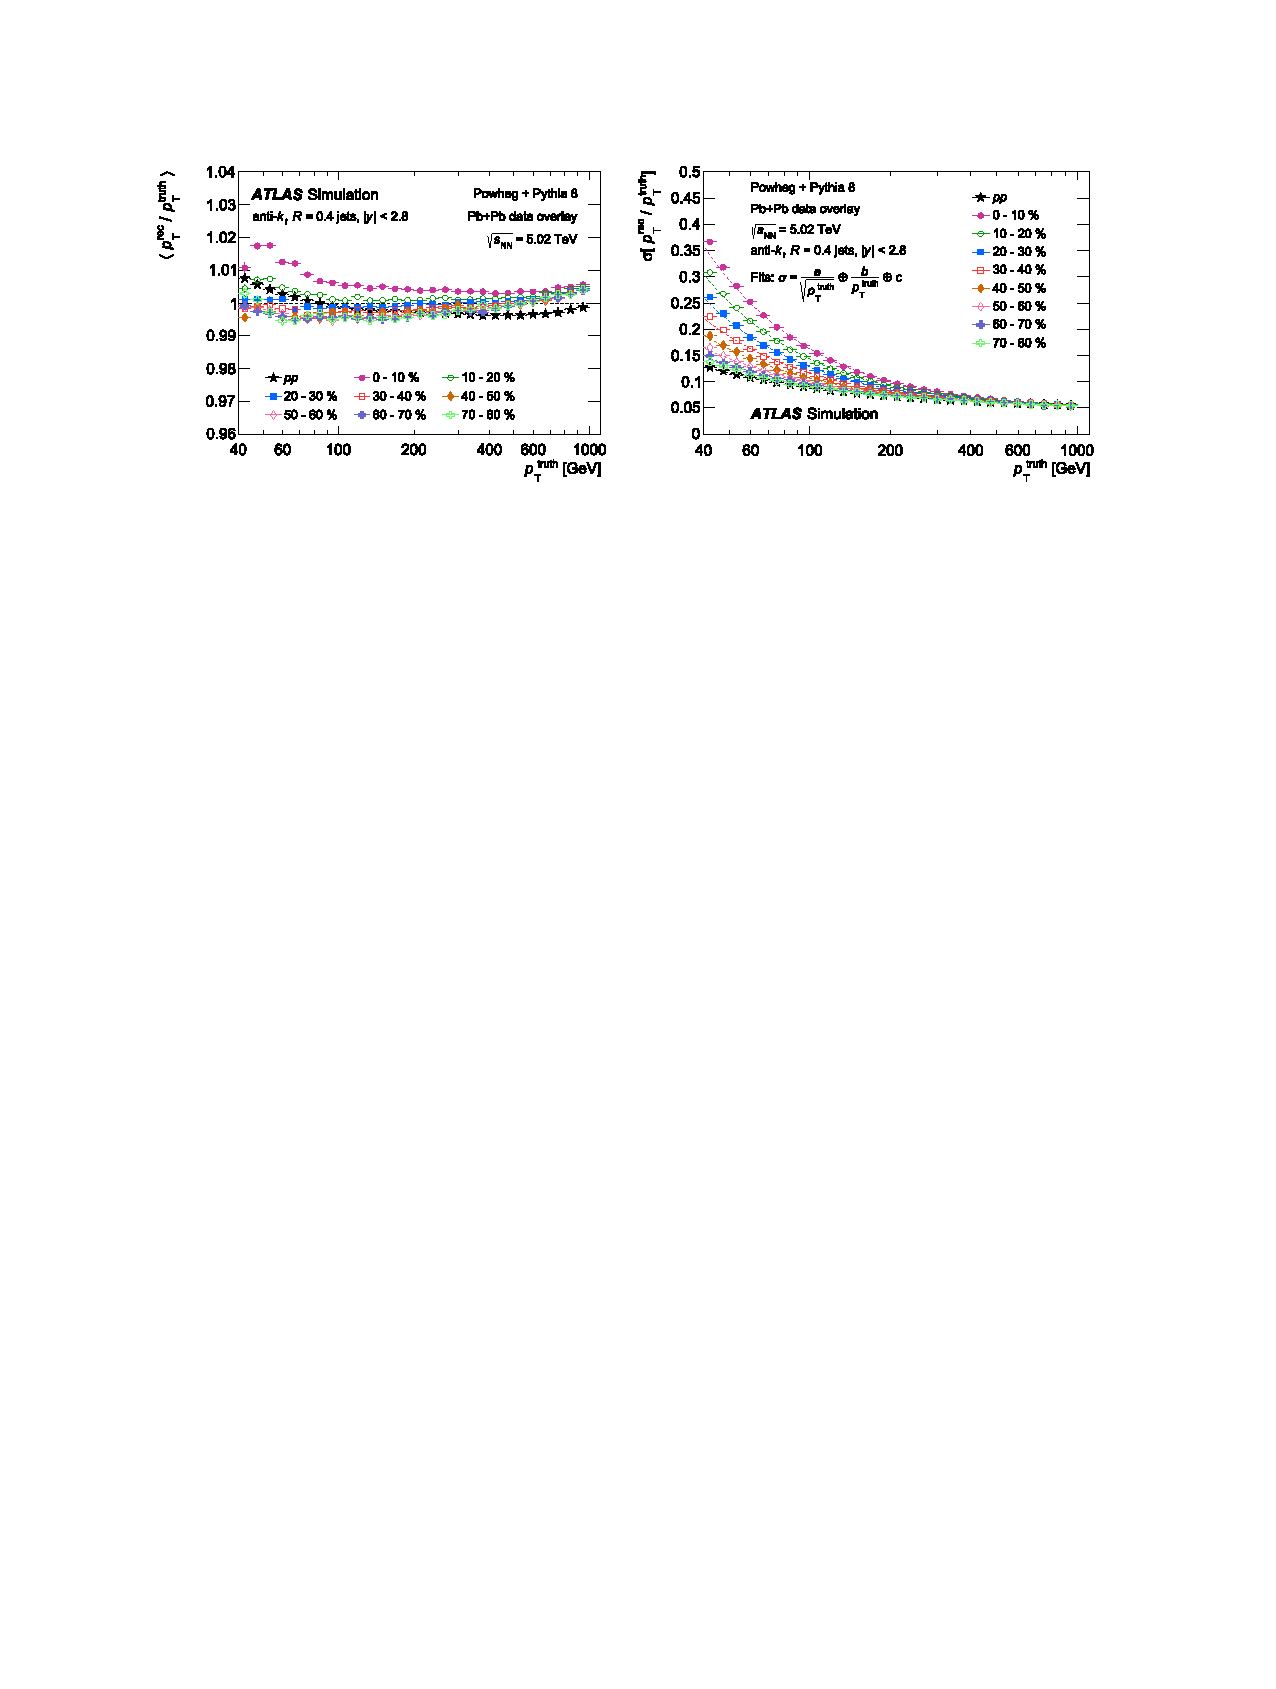
\includegraphics[width=\textwidth]{figures/setup/jes_jer} %
	\caption{
	The Jet Energy Scale (left) and Jet Energy Resolution (right) as a function of \pttruth.
	Both are for jets with $|y| < 2.8$. The different curves are for \pp\ and varying \pbpb\ centrality.
	Figures taken from \cite{2019108}.}	
	\label{fig:jes_jer}%
\end{figure}
The JES is seen to be almost unity within 1\%. across a broad kinematic range.
The JER is smaller for jets with higher transverse momentum, and depends on centrality.
It is the largest in central collisions and gets better for more peripheral collisions.
The JER can be fit to the form \cite{Aad:hi_jets}:

\begin{align}
\frac{\sigma[\Delta \Et]}{E_{\rm T}^{\rm true}} = \frac{a}{\sqrt{E_{\rm T}^{\rm true}}} \oplus \frac{b}{E_{\rm T}^{\rm true}} \oplus c
\end{align}
where $a$ and $c$ are related to the detector response.
The $b$ term describes the underlying event fluctuations and depends on centrality.
The large underlying event in central collisions results in the JER being the largest in that centrality interval. 

The $\eta$ and $\phi$ position resolution of the jet can be derived via a similar procedure and is shown in Figure~\ref{fig:jet_posResolution} as a function of the \pttruth.



\begin{figure}
\centering
\begin{subfigure}{.45\textwidth}
  \centering
  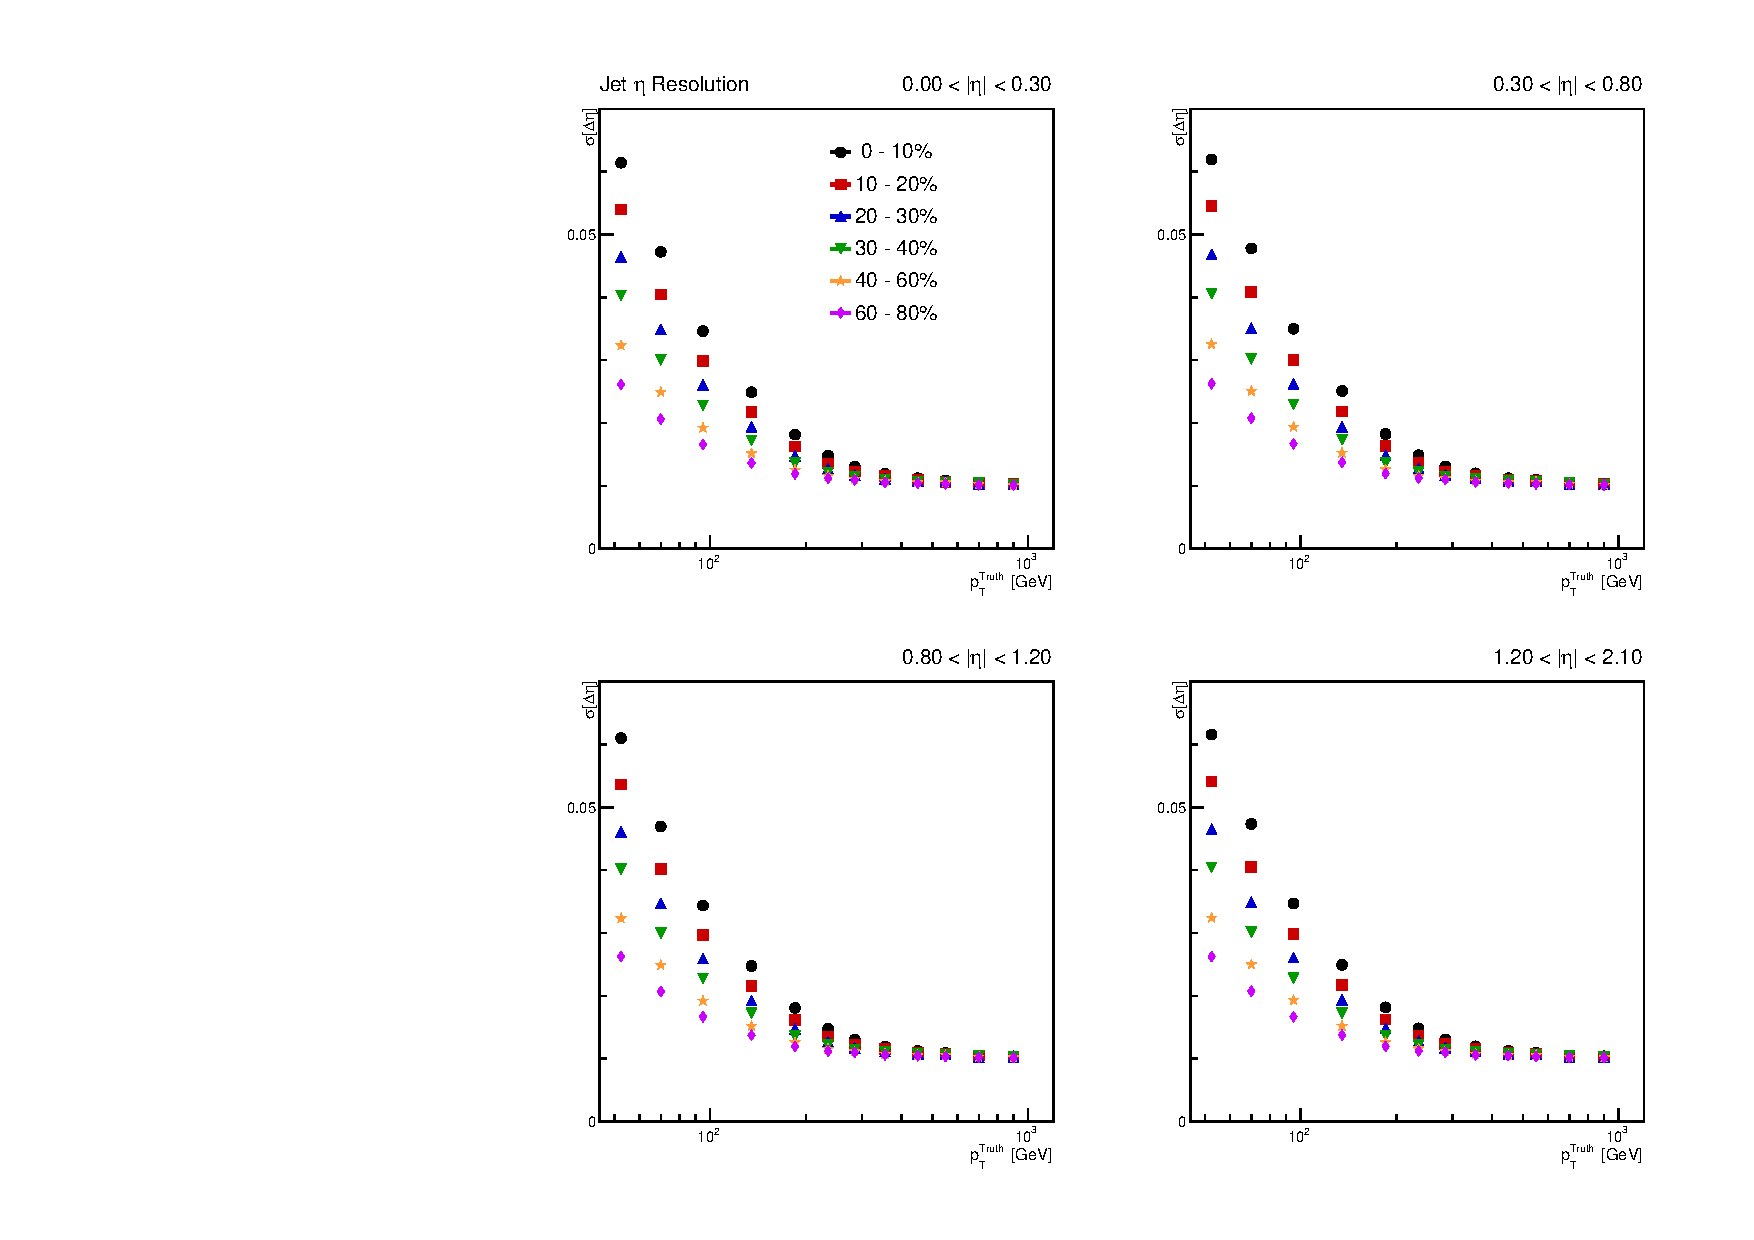
\includegraphics[width=\linewidth]{figures/setup/jet_res_eta_r04.pdf}}
          \caption{}
          \label{fig:nch_fcal}
\end{subfigure}
\qquad  \qquad  
\begin{subfigure}{.45\textwidth}  
  \centering
  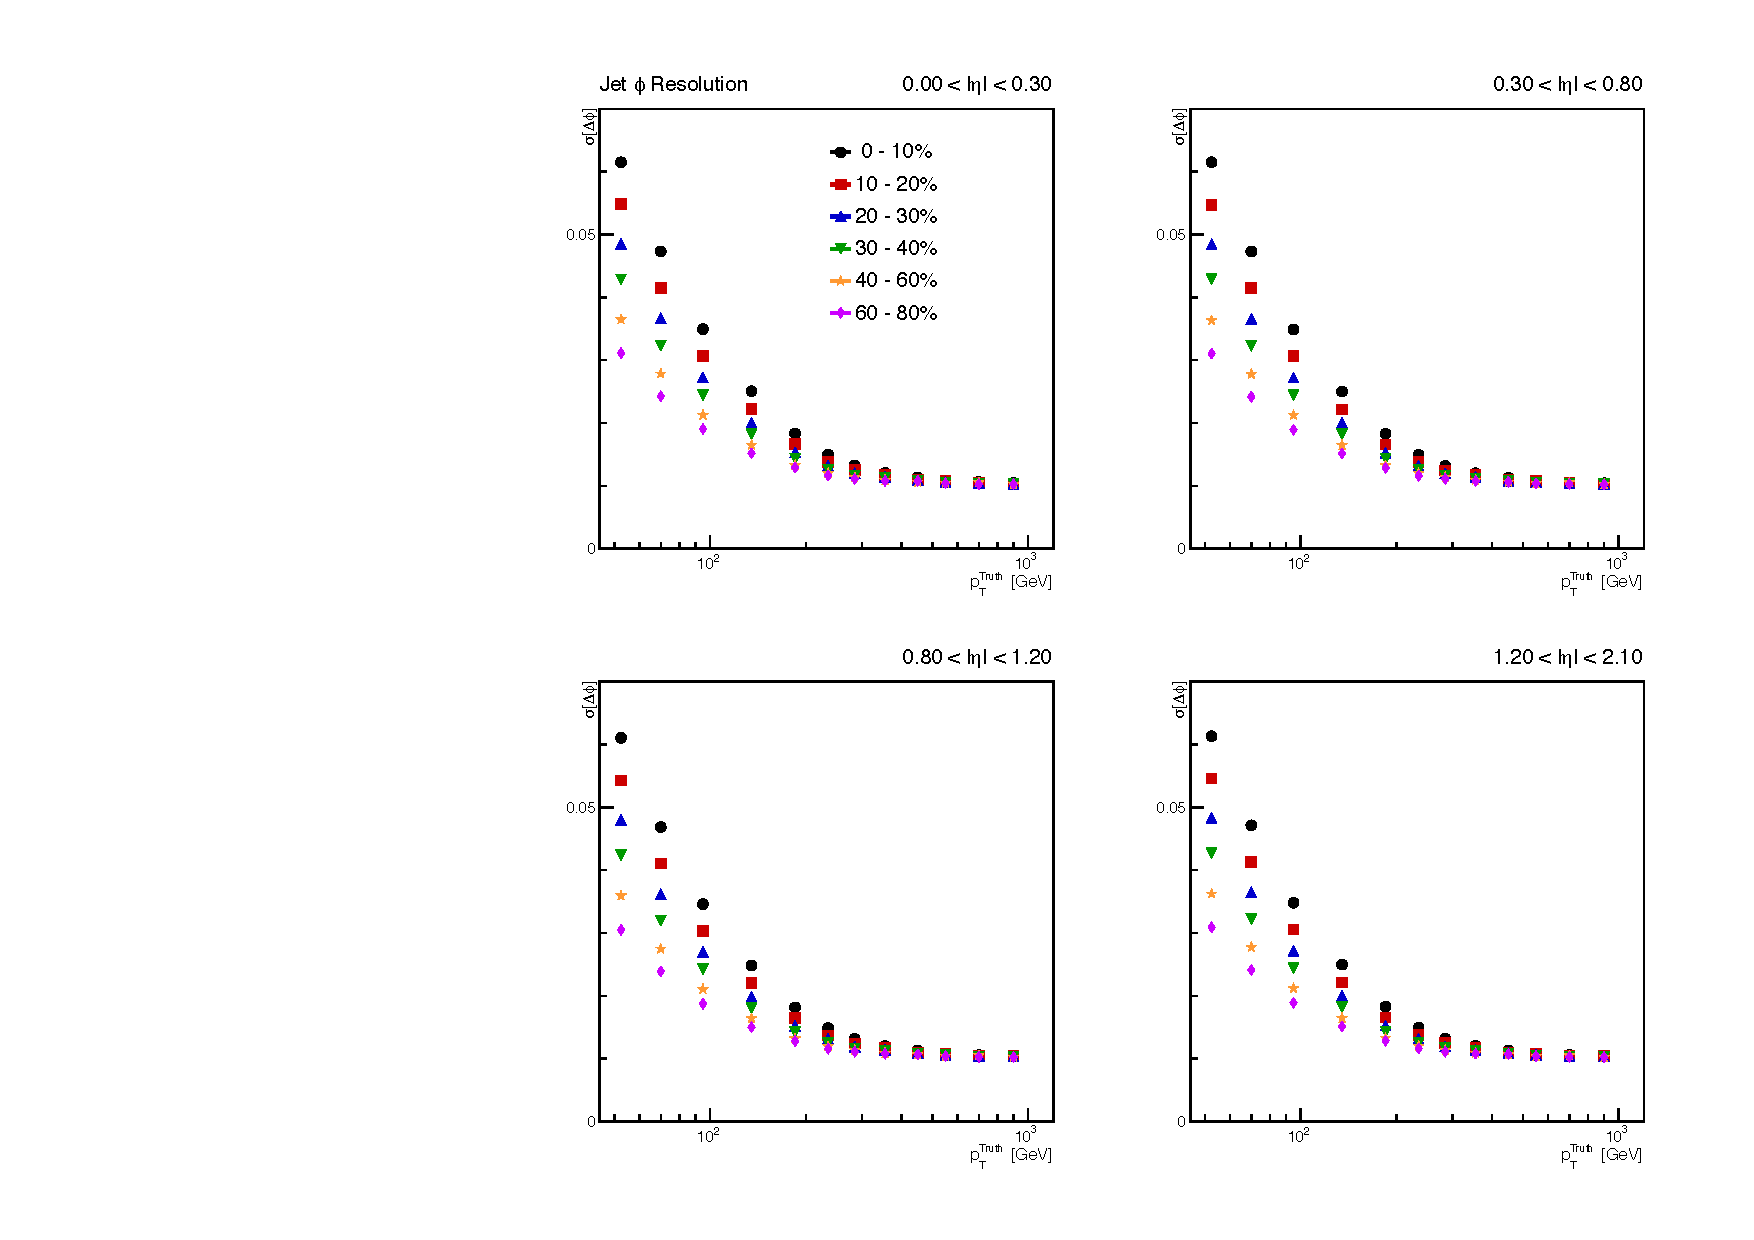
\includegraphics[width=\linewidth]{figures/setup/jet_res_phi_r04.pdf}}
          \caption{}
          \label{fig:fcal_distr}
\end{subfigure}
\caption{The (left) $\eta$ and (right) $\phi$ position resolution of the jet as a function of \pttruth\ in \pbpb\ collisions at $\sqrtsnn = 5.02$ TeV for different centrality and $\eta$ regions.
Figure taken from Ref.~\cite{Puri:2304504}.}
\label{fig:jet_posResolution}
\end{figure}




%The final corrections come from data driven (\insitu) methods like \pt\ balance studies (comparing the \pt\ of a jet and any other object like another jet, Z, or $\gamma$). Heavy ion collisions however, have the limitation that simple \pt\ balance studies are non-trivial because of jet quenching effects. Another limitation is the lack of high statistics for reference objects like $Z$'s and photons. The way to get around this is to derive a \textit{cross}-calibration, based on comparing jets in \pp\ collisions, as reconstructed by the heavy ion and \pp\ jet reconstruction algorithms. The HI jets can then be scaled with factors given by the ratio of $\langle \pt ^\hi / \pt^\emt \rangle$ in data and MC.
%
%The statistical uncertainties on the cross calibration factors come from the fits to the ratio of the relative response in data and MC, whereas the systematics come from changing the parameters of the study (these were evaluated as the maximum absolute difference between the nominal fit and any other iteration). The cross calibration factors for $0.8 < |\eta| < 1.2$, along with their uncertainties are shown on Fig.~\ref{fig:factors_w_uncertainties}. These are at the level of about 1\% and do not show strong variation with \pt. 
%\begin{figure}[htbp!]
%	\centering
%	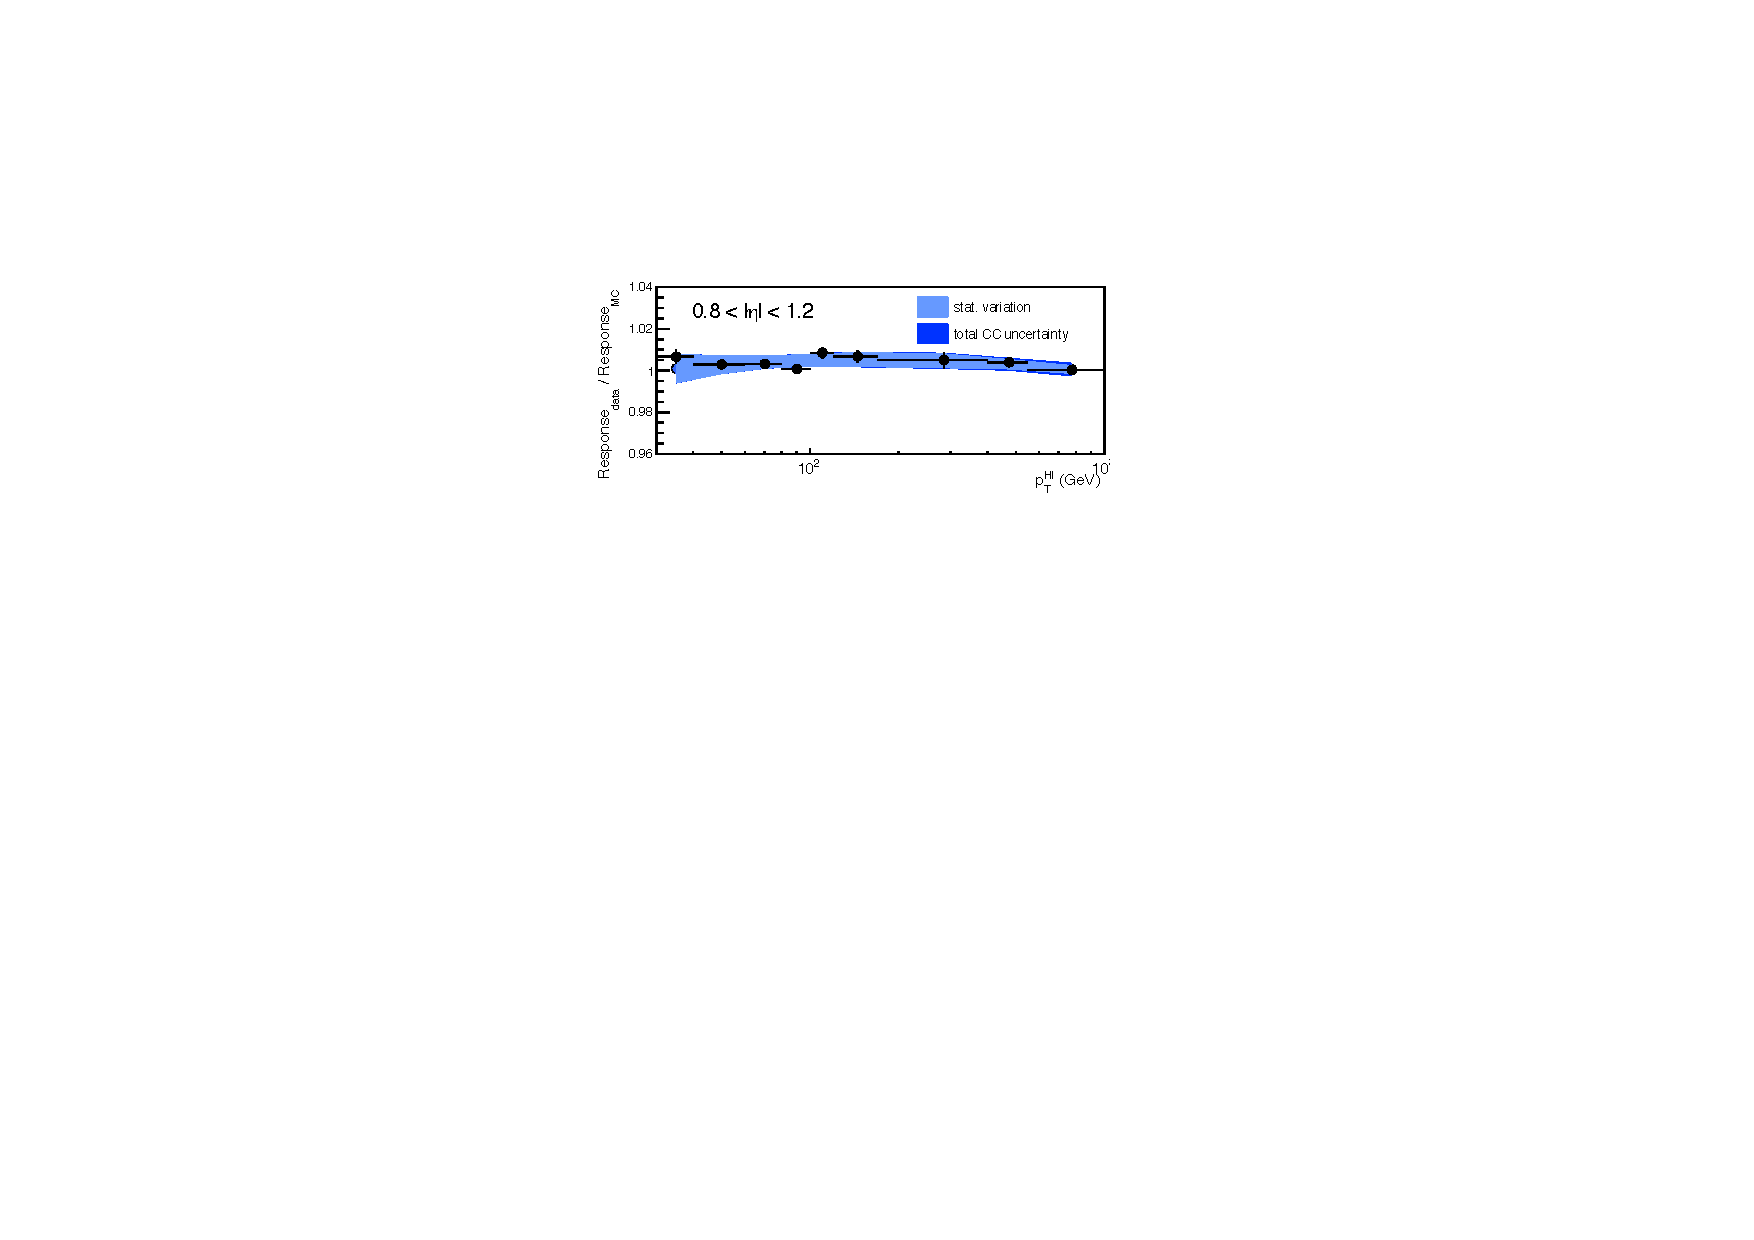
\includegraphics[width=0.5\textwidth]{figures/factors_w_uncertainties_2}
%	\caption{The cross calibration factors for $0.8 < |\eta| < 1.2$, as a function of $\textit{p}_{\text{T}}^{\text{HI}}$, along with their uncertainties.}
%	\label{fig:factors_w_uncertainties}%
%\end{figure}
%
%
%The cross-calibration procedure further allows applying the baseline jet energy scale/resolution uncertainties from the EMTopo jets, to the HI jets (along with the uncertainties of the cross-calibration procedure itself) \cite{xcalib_run1}. 
%
%
%\subsection{Heavy Ion Jet Energy Resolution Uncertainties}
%The uncertainty on the heavy ion jet energy resolution can be shown to be given by:
%
%\begin{equation}
%\delta \sigma_{\text{HI}} = \delta \sigma_{\text{EMTopo}} \sqrt{\left(1 + \frac{A}{\sigma_{\text{HI}}^2}\right)\left(1 + \left[\frac{\delta A}{2 \sigma_{\text{EMTopo}} \delta \sigma_{\text{EMTopo}}}\right)\right]^2} 
%\end{equation}
%where $\delta A ^2 = (2 s _{\text{HI}} \delta s _{\text{HI}})^2  + (2 s _{\text{EMTopo}} \delta s _{\text{EMTopo}})^2$ and $s^2_{\text{EMTopo/HI}}$ is the uncorrelated component between the errors in the jet \pt\, as reconstructed by two different algorithms applied to the same data \cite{xcalib_run1}. This result however, neglects that the uncertainty in the EMTopo jet energy resolution can be correlated with the systematic uncertainty on $A$. Accounting for this correlation, it can be shown that the uncertainty on the heavy ion jet energy resolution can be given by:
%\begin{equation}
%\dsigma_{{\text{HI}}} = \frac{\delta R_{{\text{HI}}}}{2 \sigma_{{\text{HI}}}}
%\end{equation}
%where
%\begin{align}
%R_{\text{HI}} &= \sigma_{\text{HI}}^2 \\
%\delta^2 R_{\text{HI}} &= \lambda^4 \delta^2 R_\emt + \delta^2 B \\
%\delta R_\emt  &= 2 \sigma_\emt \dsigma_\emt
%\end{align}
%Here, $\lambda$ accounts for the correlation between the HI and EMTopo jets, and $B$ is a estimate of the difference in the relative resolution between HI and EMTopo jets, as measured in data and MC.
%
%A comparison between $\delta\sigma_\emt$ and $\delta\sigma_{\text{HI}}$ can be seen in Fig.~\ref{fig:hi_jer_uncert}.
%
%
%\begin{figure}[htbp!]
%	\centering
%	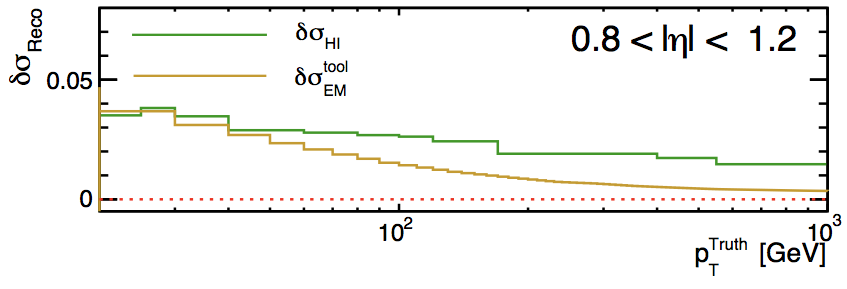
\includegraphics[width=0.7\textwidth]{uncert_2} %
%	\caption{The comparison between $\delta\sigma_\emt$ and $\delta\sigma_{\text{HI}}$ for $0.8 < |\eta| < 1.2$.}	
%	\label{fig:hi_jer_uncert}%
%\end{figure}
%
